% Copyright 2009--2010  Ed Bueler

%\section{free boundary problems}

\begin{frame}{\emph{POSTSCRIPT} on free boundary value problems}

\begin{itemize}
\item ice sheet/shelf modeling means free boundary problems
\item Hutter [1999]\nocite{HutterFreeBoundary} identifies some below
\end{itemize}
\begin{center}
  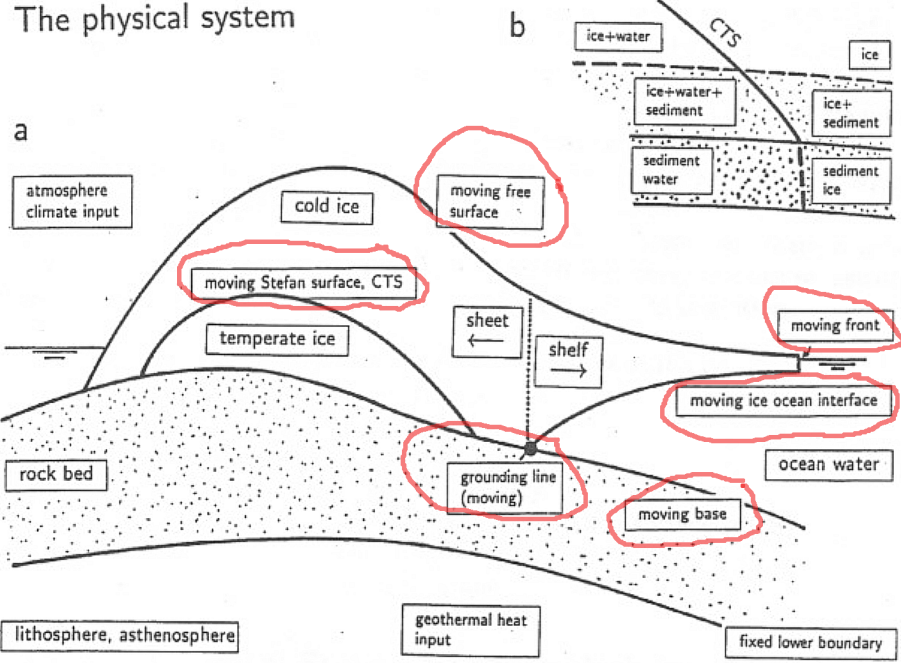
\includegraphics[width=0.8\textwidth]{photos/freehutter}
\end{center}
\end{frame}


\begin{frame}{what is a ``free boundary''?}

\begin{itemize}
\item a \emph{free boundary} for a PDE is an unknown location at which there is a boundary condition
  \begin{itemize}
  \item[$\circ$] the location of the free boundary must be found at the same time as one solves the PDE problem
  \item[$\circ$] in addition to the information which would already be present at a fixed-location boundary, there must be enough additional information at a free boundary to determine its location
  \item[$\circ$] all free boundary problems are nonlinear, regardless of the linearity of the PDE
  \end{itemize}
\item classic \emph{example}:  consider an elastic membrane attached to a wire frame and stretched over an obstacle:
\end{itemize}

\begin{columns}
\begin{column}{0.5\textwidth}
\small
constraint:
  $$u \ge \psi$$

in locations where $u>\psi$, solve:
  $$\grad^2 u = 0$$
  
\emph{where is the free boundary, and what facts about $u$ are true there?}
\end{column}
\begin{column}{0.5\textwidth}
  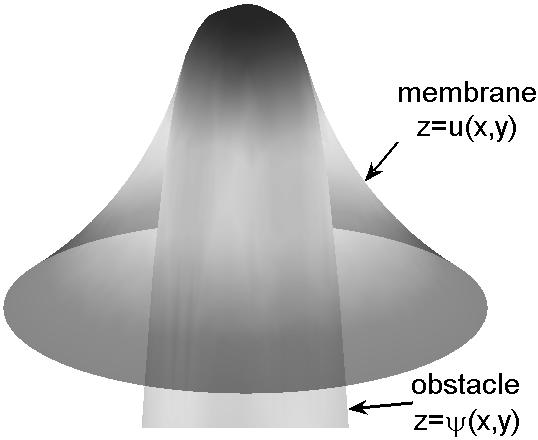
\includegraphics[width=1.0\textwidth]{photos/classicalobs}
\end{column}
\end{columns}
\end{frame}


\begin{frame}{free boundary value problem 1: polythermal ice}

\small
\begin{itemize}
\item by volume, majority of ice sheet is \emph{cold} ($T < 0\phantom{|}^\circ\text{C}$)
\item \dots but there is some ice which is \emph{temperate}, where $T = 0\phantom{|}^\circ\text{C}$ \emph{and} there is a positive liquid fraction within the ice matrix
\item \dots so ice sheets are \emph{polythermal}
\item boundary between cold and temperate ice is ``CTS'' (= cold-temperate transition surface):
  \begin{itemize}
  \item[$\circ$] must be found, as free boundary, when solving conservation of energy equation (``Stefan probem'')
  \item[$\circ$] can be tracked explicitly [Greve, 1997]\nocite{Greve}
  \item[$\circ$] or treated as a level surface of the enthalpy variable [Aschwanden and Blatter, 2009]\nocite{AschwandenBlatter}
  \end{itemize}
%\item \emph{side note}: for temperate ice there must be some dependence of ice strength (e.g.~softness $A$ in Glen law), but only one reference we can find [Lliboutry and Duval, 1985]\nocite{LliboutryDuval1985}
\end{itemize}

\begin{center}
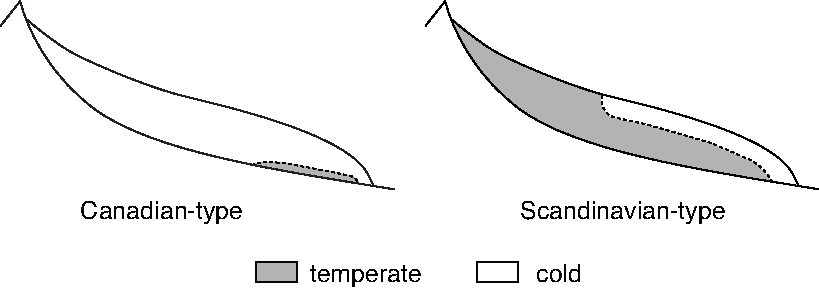
\includegraphics[width=0.8\textwidth]{photos/polythermal_types}
\end{center}
\end{frame}


\begin{frame}{free boundary value problem 2: for ice streaming}

%\vspace{-0.2in}
\begin{itemize}
\item  Schoof's [2006]\nocite{SchoofStream} insight, for diagnostic case
  $$\text{SSA + (plastic till)} = \begin{pmatrix}
\text{well-posed free boundary problem} \\ \text{for location \emph{and} velocity of sliding}
\end{pmatrix} $$
\item ``plastic till'' means the basal strength (resistance) is given by a yield stress $\tau_c$:  \qquad $\vec\tau_b = \tau_c \mathbf{v}_b / |\mathbf{v}_b|$
\item Schoof's scheme is a \emph{whole ice sheet form} of MacAyeal's [1989]\nocite{MacAyeal} individual ice stream models
\end{itemize}

\mode<presentation>
{
\begin{columns}
\begin{column}{0.5\textwidth}
\begin{center}
  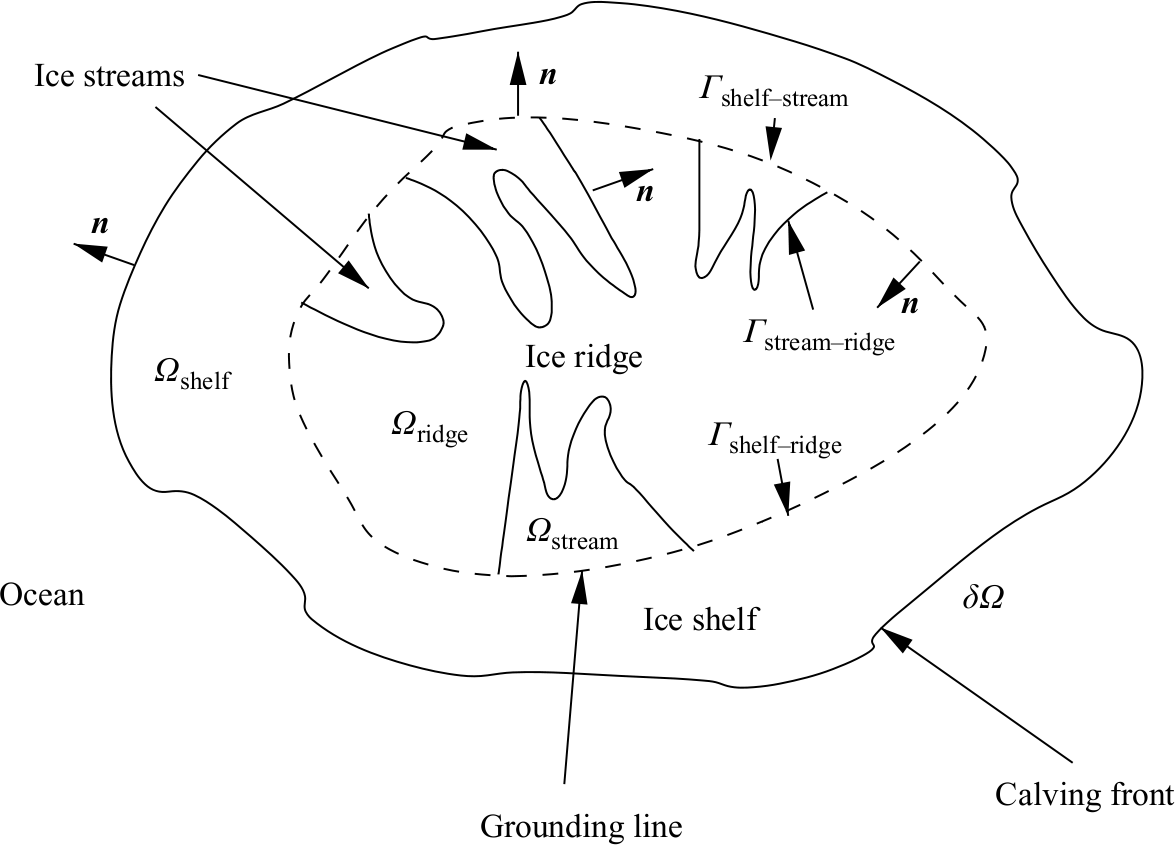
\includegraphics[width=1.0\textwidth]{photos/schoof_planform}
\end{center}
\end{column}
\begin{column}{0.5\textwidth}
\begin{center}
  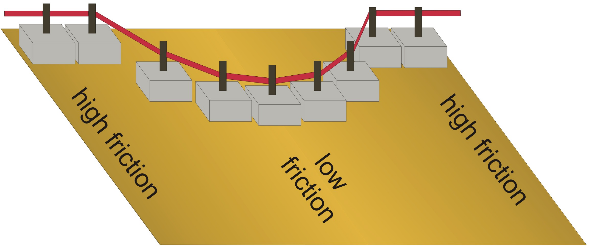
\includegraphics[width=0.95\textwidth]{photos/schoof_sliders}
\end{center}
\end{column}
\end{columns}
}
\mode<article>
{
  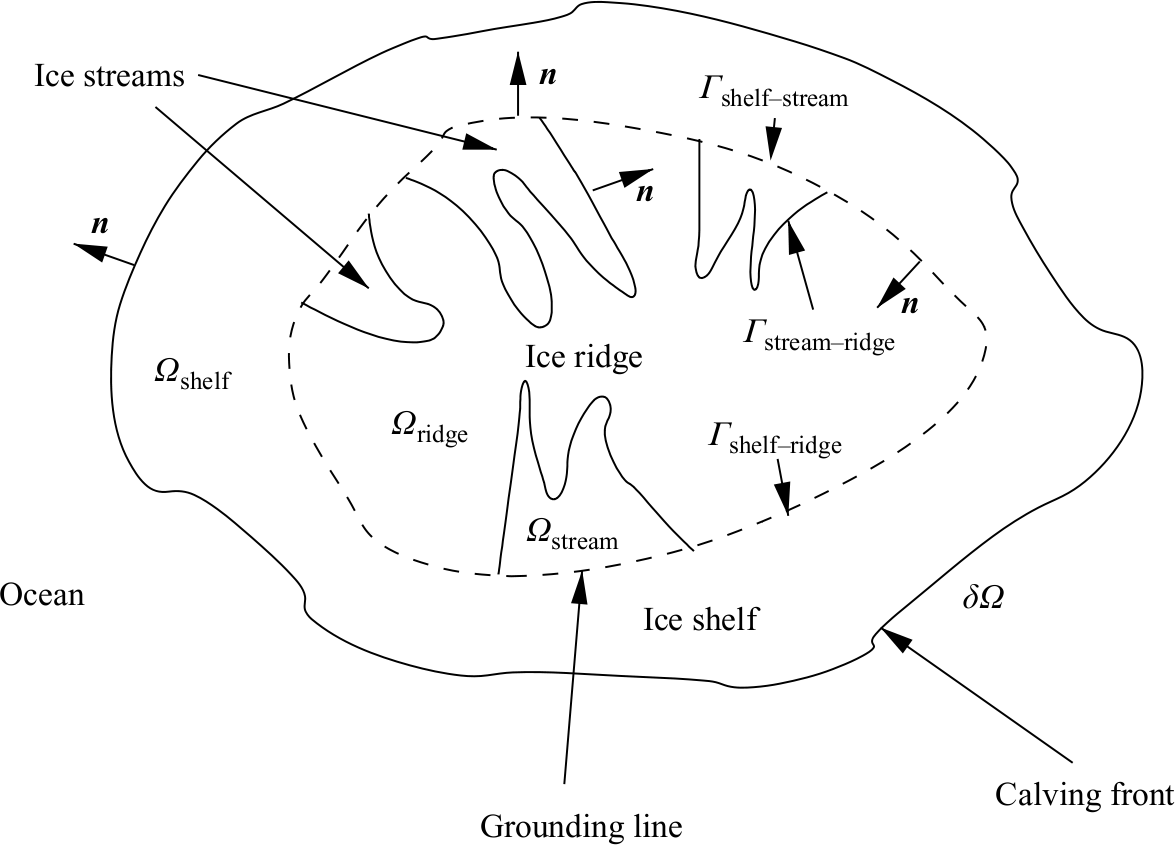
\includegraphics[width=0.7\textwidth]{photos/schoof_planform} \qquad
  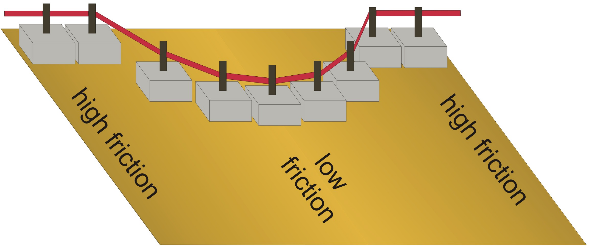
\includegraphics[width=0.45\textwidth]{photos/schoof_sliders}
}
\end{frame}


\begin{frame}{free boundary problem 3: for grounded ice sheet margin}

\begin{itemize}
\item side-by-side comparison, \emph{classical elastic membrane problem} versus \emph{steady ice sheet problem}
\end{itemize}
\small
\begin{columns}[T]
\begin{column}{0.4\textwidth}
constraint:
  $$u \ge \psi$$

where $u>\psi$, solve:
  $$\grad^2 u = 0$$

\bigskip
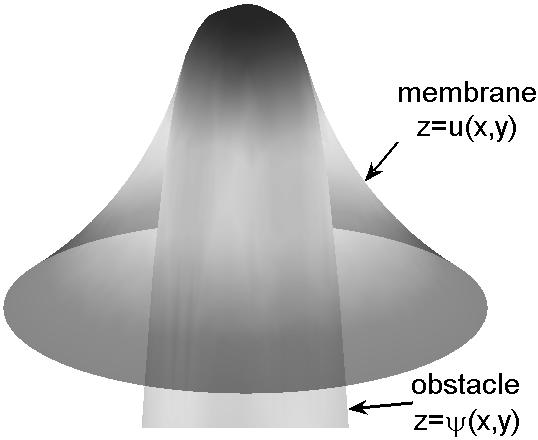
\includegraphics[width=0.8\textwidth]{photos/classicalobs}
\end{column}
\begin{column}{0.6\textwidth}
constraint:
  $$h \ge b \qquad \iff \qquad H \ge 0$$

where $h>b$, solve steady SIA:
  $$0 = M + \Div \left(\Gamma H^{n+2} |\grad h|^{n-1} \grad h \right)$$

\bigskip
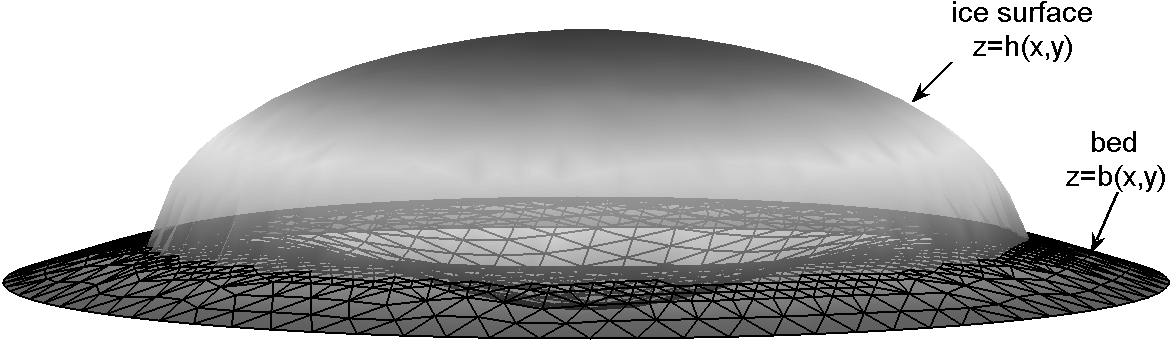
\includegraphics[width=0.9\textwidth]{photos/capnonflatobs}
\end{column}
\end{columns}
\end{frame}


\begin{frame}{for SIA model, an illuminating transformation}

\begin{itemize}
\item there are degenerate diffusions in other fields
\item (e.g.~porous media where there can be wet and dry parts)
\item \dots whence transformations useful to ice sheet modeling
\item specifically one by Raviart [1970]\nocite{Raviart} \scriptsize($n=3$ case)\normalsize:\qquad $\eta = H^{8/3}$
\item the \emph{flat bed} SIA simplifies:
	$$H_t = M + \Div \left({\color{red}\Gamma H^5 |\grad H|^2}\, \grad H \right)$$
	$$\quad \stackrel{\text{becomes}}{\to} \quad  \left(\eta^{3/8}\right)_t = M + \Div ({\color{red}\tilde\Gamma |\grad \eta|^2}\, \grad \eta)$$
  \begin{itemize}
  \item[$\circ$] new diffusivity ({\color{red}red}) depends on $|\grad \eta|$ only, not $\eta$
  \item[$\circ$] the margin shape is not singular in new variable!
     \begin{itemize}
     \item[$\ast$]  $\grad \eta$ is globally continuous
     \item[$\ast$] $z=\eta(t,x,y)$ is tangent to bed at margin
     \end{itemize}
  \item[$\circ$] numerical methods applied to the new equation make errors which are as expected for ``good'' free boundary problems [Bueler and others, 2005]\nocite{BLKCB}
  \end{itemize}
\end{itemize}
\end{frame}


% THIS IS AN ABSTRACTION TOO FAR:
%\begin{frame}{the 3 point ice sheet}
%\begin{itemize}
%\item new view of boundary conditions
%\item free boundary problem as inequality
%\item geometrization
%\end{itemize}
%\end{frame}


\begin{frame}{free boundary problems: \emph{so what}?}
\begin{itemize}
\item why does it matter that many glaciological problems are free boundary problems in their mathematical form?
\item the location of the free boundary may \emph{be} the glaciological question
\item free boundaries are always locations of \emph{loss of smoothness} relative to fixed boundary solutions
     \begin{itemize}
     \item[$\circ$] numerical error may be dominated by errors near these free boundaries, 
     \item[$\circ$] hard to know whether model results at free boundaries are poor because of numerical problems or because of missing physical processes
     \end{itemize}
\end{itemize}
\end{frame}
